\documentclass{article}

\usepackage[english, russian]{babel}
\usepackage{geometry}
\usepackage{graphicx}
\usepackage{listings}
\usepackage{xcolor}
\usepackage[14pt]{extsizes}
\usepackage{amsmath}
\usepackage{setspace}
\usepackage{multirow}
\usepackage{tocloft}
\usepackage{indentfirst} 

\renewcommand{\cftsecleader}{\cftdotfill{\cftdotsep}}
\geometry{pdftex, left = 3cm, right = 1cm, top = 2cm, bottom = 2cm}
\onehalfspacing

\lstdefinestyle{python}{
	language={Python},
	basicstyle=\footnotesize\ttfamily,
	numbers=left,
	frame=single,
	tabsize=4,
	breaklines=true
}

\begin{document}
\begin{titlepage}
	\newgeometry{pdftex, left=2cm, right=2cm, top=2.5cm, bottom=2.5cm}
	\fontsize{12pt}{12pt}\selectfont
	\noindent\begin{tabular}{|c|c|}	\hline
	\noindent\begin{minipage}{0.15\textwidth}
		
\includegraphics[width=\linewidth]{tools/logo.png}
	\end{minipage} &
	\noindent\begin{minipage}{0.85\textwidth}\centering
		\textbf{\newline Министерство науки и высшего образования Российской Федерации}\\
		\textbf{Федеральное государственное бюджетное образовательное учреждение высшего образования}\\
		\textbf{«Московский государственный технический университет имени Н.Э.~Баумана}\\
		\textbf{(национальный исследовательский университет)»}\\
		\textbf{(МГТУ им. Н.Э.~Баумана)}
	\end{minipage} \\
	\hline	\end{tabular}\newline\newline\newline
	\noindent ФАКУЛЬТЕТ \underline{«Информатика и системы управления»} \newline\newline
	\noindent КАФЕДРА \underline{«Программное обеспечение ЭВМ и информационные технологии»}\newline\newline\newline\newline\newline\newline

	\noindent\begin{minipage}{1.0\textwidth}\centering
		\Large\textbf{   ~~~ Лабораторная работа №1}\newline
		\textbf{по дисциплине "Анализ алгоритмов"}\newline\newline\newline\newline\newline
	\end{minipage}

	\noindent\textbf{Тема} \underline{Алгоритмы Левенштейна и Дамерау-Левенштейна}\newline\newline
	\textbf{Студент} \underline{Тузов Даниил Александрович}\newline\newline
	\textbf{Группа} \underline{ИУ7-52Б}\newline\newline
	\textbf{Преподаватель} \underline{Строганов Дмитрий Владимирович}
	
	\begin{center}
		\vfill
		Москва, \the\year ~г.
	\end{center}
	\restoregeometry
	\clearpage
\end{titlepage}

\renewcommand{\contentsname}{Содержание} 
\tableofcontents
\setcounter{page}{2}
\clearpage

\section*{Введение}
\addcontentsline{toc}{section}{ВВЕДЕНИЕ}
В первой лабораторной работе по анализу алгоритмов рассматривается понятие расстояния Левенштейна. 
Это самое расстояние показывает минимальное количество операций вставки, удаления и замены, которое 
необходимо для преобразования первой строки во вторую.

Целью лабораторной работы является изучение алгоритмов нахождения расстояния Левенштейна.
Для достижения поставленной цели небходимо решить следующие задачи:
\begin{itemize}
	\item изучить понятие расстояния Левенштейна и расстояние Дамерау-Левенштейна
	\item реализовать алгоритмы для нахождения искомого расстояния:
	\begin{itemize}
		\item рекурсивный алгоритм
		\item рекурсивный алгоритм с кэшированием
		\item нерекурсивный алгоритм, основанный на динамическом программировании
		\item алгоритм нахождения расстояния Дамерау-Левенштейна
	\end{itemize}
	\item сравнить алгоритмы по затраченному процессорному времени и памяти
	\item обосновать полученные результаты
\end{itemize}


\clearpage\section{Аналитическая часть}
В этой части рассматриваются теоретические аспекты понятия расстояния между строками на примере алгоритмов 
Левенштейна и Дамерау-Левенштейна.

\subsection{Расстояние Левенштейна}
Расстояние Левенштейна [4] -- минимальное количество операций вставки, удаления и замены, необходимых для
преобразования одной строки в другую. 

Расстояние Левенштейна D($S_{1}$, $S_{2}$) для строк $S_{1}$ и $S_{2}$ можно найти  по формуле \ref{eq:Lev}:

\begin{equation}
	\label{eq:Lev}
	D(i, j) = \begin{cases}
	i, &\text{j = 0, i > 0}\\
	j, &\text{i = 0, j > 0}\\
	D(i - 1, j - 1), &\text{i > 0, j > 0, $S_{1}[i] = S_{2}[j]$}\\
	1 + min \begin{cases}
		D(i, j - 1)\\
		D(i - 1, j)\\
		D(i - 1, j - 1)\\
	\end{cases}, &\text{i > 0, j > 0, $S_{1}[i] \neq S_{2}[j]$}
	\end{cases}
\end{equation}

где i и j -- индексы в строках $S_{1}$ и $S_{2}$.

\subsection{Возможные реализации}
Поскольку алгоритм Левенштейна задается рекурентной формулой, то одной из возможных реализаций
является рекурсия. Однако при рекурсивной реализации возможны множественные рекурсивные вызовы
с одинаковыми параметрами. Это можно предотвратить, если ввести кэш-матрицу, в которую будут заносится
уже вычисленные значения. Затем они используются при повторяющихся рекурсивных вызовах. Возможна также 
нерекурсивная реализация с помощью динамического программирования. Все алгоритмы подробнее будут
описаны в следующей части.

\subsection{Расстояние Дамерау-Левенштейна}
Для вычисления расстояния Дамерау-Левенштейна [4] необходимо дополнительно учитывать операцию обмена
двух соседних символов.

Это расстояние D($S_{1}$, $S_{2}$) для строк $S_{1}$ и $S_{2}$ можно найти  по формуле \ref{eq:DLev}:

\begin{equation}
	\label{eq:DLev}
	D(i, j) = \begin{cases}
	i, &\text{j = 0, i > 0} \\
	j, &\text{i = 0, j > 0} \\
	D(i - 1, j - 1), &\text{i > 0, j > 0, $S_{1}[i] = S_{2}[j]$} \\
	1 + min \begin{cases}
		D(i, j - 1)\\
		D(i - 1, j)\\
		D(i - 1, j - 1) \\
		D(i - 2, j - 2) \\
	\end{cases}, &\text{ $S_{1}[i] = S_{2}[j - 1],  S_{1}[i - 1] = S_{2}[j]$}\\
	1 + min \begin{cases}
		D(i, j - 1)\\
		D(i - 1, j)\\
		D(i - 1, j - 1)\\
	\end{cases}, &\text{иначе}
	\end{cases}
\end{equation}

где i и j -- индексы в строках $S_{1}$ и $S_{2}$.

\subsection{Вывод}
В этой части были рассмотрены теоретические аспекты алгоритмов нахождения расстояния между строками -- 
алгоритмов Левенштейна и Дамерау Левенштейна. Алгоритмы в этом разделе представлены рекурентными
формулами. В последующих разделах будет рассматриваться 4 реализации алгоритмов: рекурсивный алгоритм 
Левенштейна, рекурсивный алгоритм Левенштейна с кэшированием данных, алгоритм Левенштейна, основанный 
на динамическом программировании и алгоритм Дамерау-Левенштейна, основанный на динамическом 
программировании.


\clearpage\section{Конструкторская часть}
В этой части представлены схемы алгоритмов.

\subsection{Схемы алгоритмов}
На вход алгоритмам подаются строки $S_{1}$ и $S_{2}$ (в реализации с кэширование подается еще и кэш-матрица), на 
выходе единственное число -- искомое расстояние.

На рисунках \ref{fig:rec_lev} - \ref{fig:dlev} приведены схемы алгоритмов.

\begin{figure}[h]
	\centering
	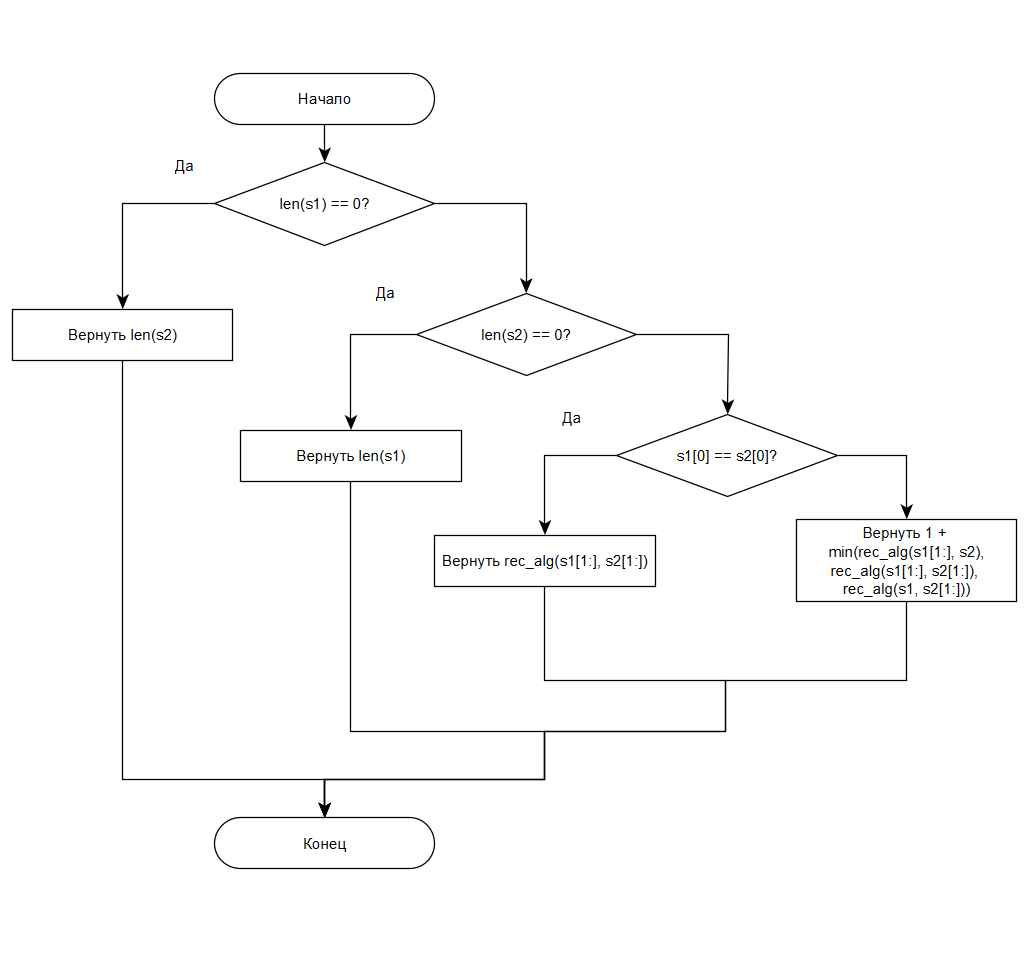
\includegraphics[scale=0.7]{tools/alg_1.png}
	\caption{Схема рекурсивного алгоритма нахождения расстояния Левенштейна}
	\label{fig:rec_lev}
\end{figure}

\begin{figure}[h]
	\centering
	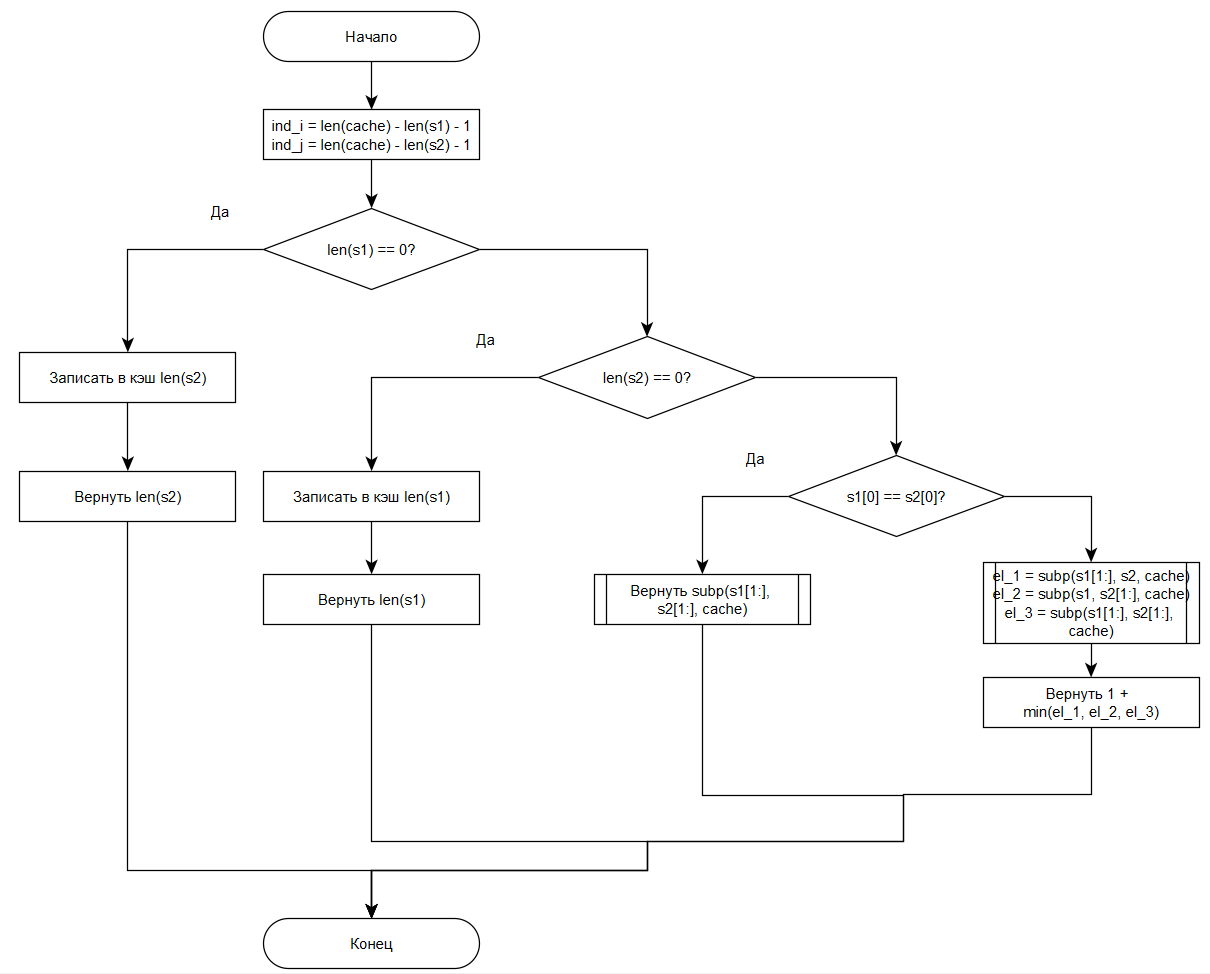
\includegraphics[scale=0.7]{tools/alg_2.png}
	\caption{Схема рекурсивного алгоритма нахождения расстояния Левенштейна с кэшированием}
	\label{fig:rec_lev_cache}
\end{figure}

\begin{figure}[h]
	\centering
	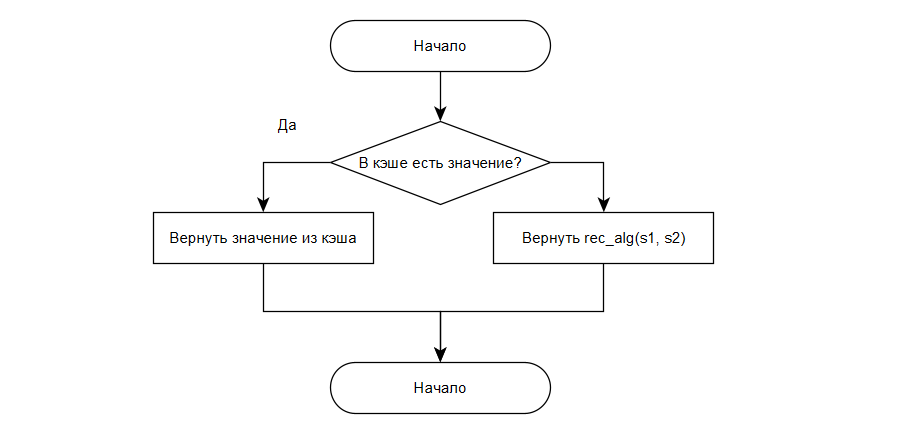
\includegraphics[scale=1.0]{tools/alg_2_subp.png}
	\caption{Схема подпрограммы subp, вызываемой в алгоритме с кэшированием}
	\label{fig:rec_lev_cache_subp}
\end{figure}

\begin{figure}[h]
	\centering
	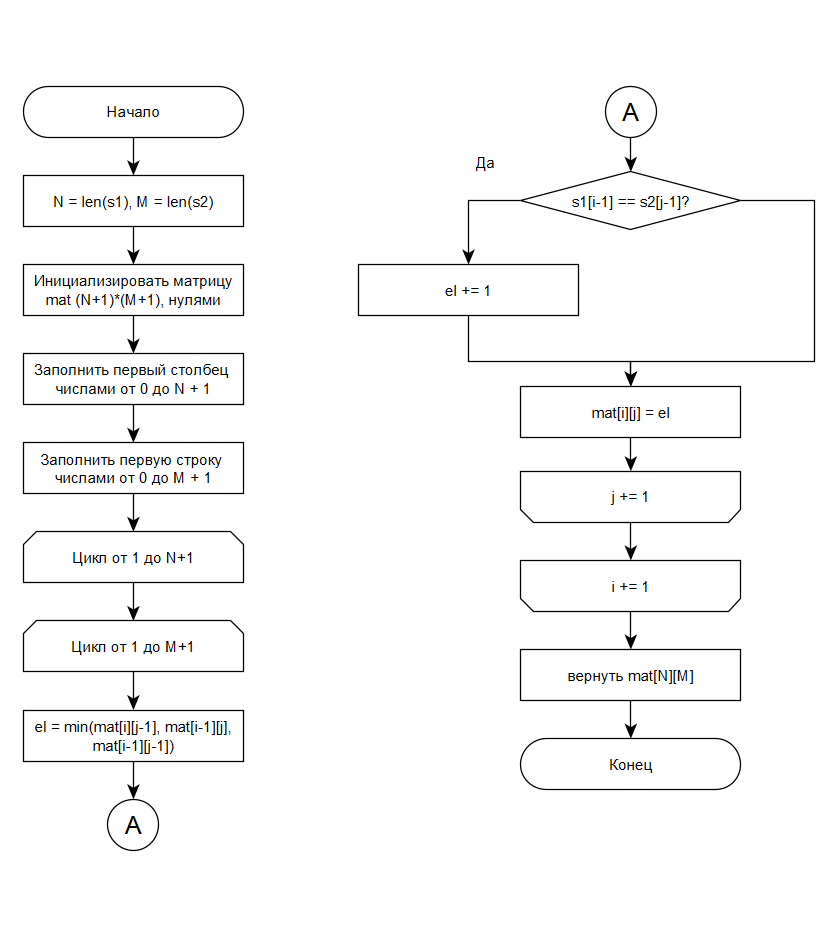
\includegraphics[scale=0.9]{tools/alg_3.png}
	\caption{Схема нерекурсивного алгоритма нахождения расстояния Левенштейна}
	\label{fig:lev}
\end{figure}

\begin{figure}[h]
	\centering
	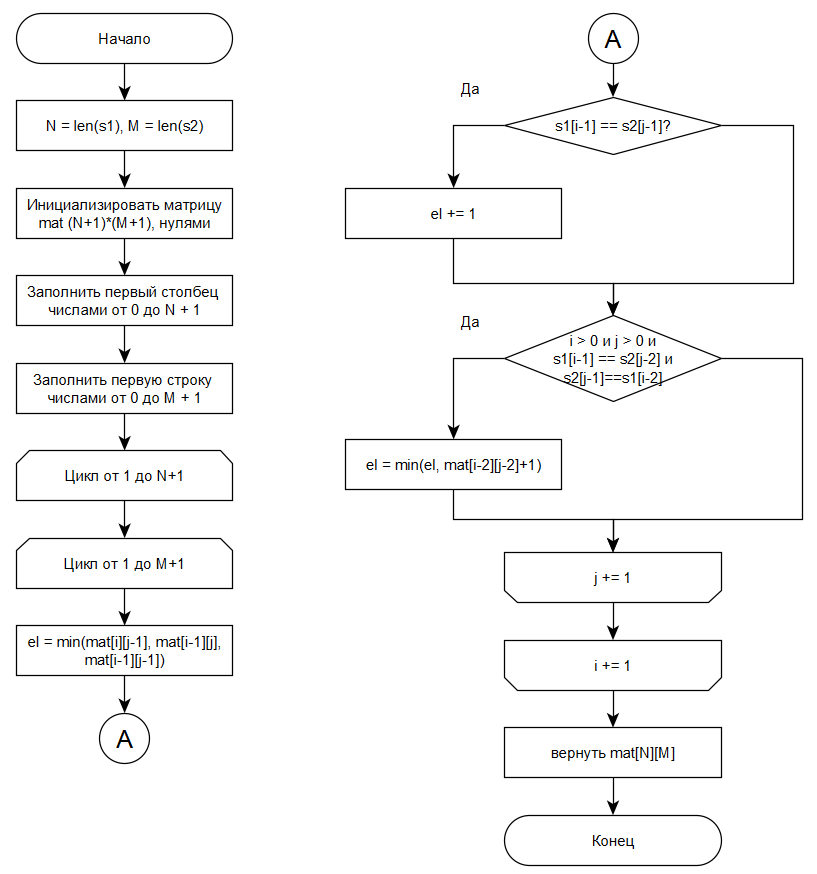
\includegraphics[scale=0.9]{tools/alg_4.png}
	\caption{Схема нерекурсивного алгоритма нахождения расстояния Дамерау-Левенштейна}
	\label{fig:dlev}
\end{figure}

\clearpage\subsection{Вывод}
В этом разделе на основе теоретических аспектов были представлены схемы рекурсивного алгоритма, рекурсивного алгоритма
с кэшированием, нерекурсивного алгоритма, основанного на динамическом программировании, а также схема алгоритма
Дамерау-Левенштейна.


\clearpage\section{Технологическая часть}
В этом разделе обоснованы средства реализации, а так же представлены листинги кодов алгоритмов и функциональные тесты.

\subsection{Средства реализации}
Для реализации алгоритмов в этой лабораторной работы был выбран язык $Python$ [2], потому что он прост в
работе, а также в нем нет автоматического сборщика мусора. Время работы было замерено с помощью функции
\textit{process\_time} [1] из библиотеки $time$. [3]

\subsection{Листинги кодов алгоритмов}
В листингах \ref{lst:rec_alg} - \ref{lst:damerau_alg} представлены коды написанных алгоритмов.

\begin{lstlisting}[style=python, label=lst:rec_alg,caption=Рекурсивный алгоритм]
def lev_recursion(s1, s2, output = False):
    len1 = len(s1)
    len2 = len(s2)

    if len1 == 0 or len2 == 0:
        return abs(len1 - len2)

    m = 0 if s1[-1] == s2[-1] else 1

    return min(lev_recursion(s1,      s2[:-1]) + 1,
               lev_recursion(s1[:-1], s2     ) + 1,
               lev_recursion(s1[:-1], s2[:-1]) + m)
\end{lstlisting}

\clearpage\begin{lstlisting}[style=python, label=lst:cache_alg,caption=Рекурсивный алгоритм с кэшированием]
def cache_alg(s1, s2, cache_mat):
    ind_i = len(cache_mat) - len(s1) - 1
    ind_j = len(cache_mat[0]) - len(s2) - 1
    if len(s1) == 0:
        cache_mat[ind_i][ind_j] = len(s2)
        return len(s2)
    elif len(s2) == 0:
        cache_mat[ind_i][ind_j] = len(s1)
        return len(s1)
    elif s1[0] == s2[0]:
        el = cache_mat[ind_i + 1][ind_j + 1]
        return el if el != -1 else cache_alg(s1[1:], s2[1:], cache_mat)

    el_1 = cache_mat[ind_i + 1][ind_j]
    el_2 = cache_mat[ind_i][ind_j + 1]
    el_3 = cache_mat[ind_i + 1][ind_j + 1]
    return 1 + min(el_1 if el_1 != -1 else cache_alg(s1[1:], s2, cache_mat),
                   el_2 if el_2 != -1 else cache_alg(s1, s2[1:], cache_mat),
                   el_3 if el_3 != -1 else cache_alg(s1[1:], s2[1:], cache_mat))
\end{lstlisting}

\begin{lstlisting}[style=python, label=lst:dp_alg,caption=Нерекурсивный алгоритм]
def DP_alg(s1, s2):
    n = len(s1)
    m = len(s2)
    matrix = [[0 for j in range(m + 1)] for i in range(n + 1)]
    for i in range(m + 1):
        matrix[0][i] = i

    for i in range(n + 1):
        matrix[i][0] = i

    for i in range(1, n + 1):
        for j in range(1, m + 1):
            el = min(matrix[i - 1][j],
                     matrix[i - 1][j - 1],
                     matrix[i][j - 1])
            if s1[i - 1] != s2[j - 1]:
                el += 1
            matrix[i][j] = el

    return matrix[-1][-1]
\end{lstlisting}

\begin{lstlisting}[style=python, label=lst:damerau_alg,caption=Нерекурсивный алгоритм Дамерау-Левенштейна]
def damerau_alg(s1, s2):
    n = len(s1)
    m = len(s2)
    matrix = [[0 for j in range(m + 1)] for i in range(n + 1)]
    for i in range(m + 1):
        matrix[0][i] = i

    for i in range(n + 1):
        matrix[i][0] = i

    for i in range(1, n + 1):
        for j in range(1, m + 1):
            el = min(matrix[i - 1][j],
                     matrix[i - 1][j - 1],
                     matrix[i][j - 1])
            if s1[i - 1] != s2[j - 1]:
                el += 1
            if i > 1 and j > 1 and s1[i - 1] == s2[j - 2] and s1[i - 2] == s2[j  - 1]:
                el = min(el, matrix[i - 2][j - 2] + 1)
            matrix[i][j] = el

    return matrix[-1][-1]
\end{lstlisting}

\clearpage\subsection{Функциональные тесты}
В таблице \ref{tbl:func_test} приведены функциональные тесты, на которых тестировалась программа.
\begin{table}[h]
	\begin{center}
	\caption{\label{tbl:func_test} Функциональные тесты}
	\begin{tabular}{|c|c|c|c|}
		\hline
		$S_{1}$ & $S_{2}$ & Левенштейн &  Дамерау-Левенштейн
		\\ \hline
		а & [] & 1 & 1  
		\\ \hline
		[] & [] & 0 & 0                             
		\\ \hline
		а & б & 1 & 1 
		\\ \hline
		а & аб & 1 & 1 
		\\ \hline
		река & мука & 2 & 2 
		\\ \hline
		реак & мука & 4 & 3 
		\\ \hline
		морковка & сосиска & 5 & 5 
		\\ \hline
		река & мука & 2 & 2 
		\\ \hline
		мамам & мамам & 0 & 0 
		\\ \hline
	\end{tabular}
	\end{center}
\end{table}

\subsection{Вывод}
В этом разделе на основе схем алгоритмов были написаны и представлены листинги кода. Помимо алгоритмов
представлены функциональные тесты, на которых был протестирован каждый алгоритм.


\clearpage\section{Исследовательская часть}
В этом разделе приведено сравнение по времени и по памяти написанных алгоритмов.

\subsection{Технические характеристики ЭВМ}
Все замеры проводились на ЭВМ, характеристики которой приведены ниже:
\begin{itemize}
	\item Процессор -- 12th Gen Intel(R) Core(TM) i5-12450H   2.00 GHz
	\item Оперативная память -- 16,0 ГБ
	\item Тип системы -- 64-разрядная операционная система, процессор x64
	\item Операционная система -- Windows 11
	\item Версия ОС -- 23H2
\end{itemize}

\subsection{Сравнение  по времени}
Время выполнения работы алгоритмов представлено в секундах. Проводилось 150 замеров.

\begin{table}[h]
	\begin{center}
	\caption{\label{tbl:all_time_cmp} Сравнение алгоритмов по времени выполнения}
	\begin{tabular}{|c|c|c|c|c|}
		\hline
		Размер строк & Рекурсивный & C кэшем &  Нерекурсивный & Дамерау
		\\ \hline
		1 & 0 & 0 & 0 & 0
		\\ \hline
		2 & 0 & 0 & 0 & 0
		\\ \hline
		3 & 0 & 0 & 0 & 0
		\\ \hline
		4 & 0 & 0 & 0 & 0
		\\ \hline
		5 & 0 & 0.001 & 0 & 0
		\\ \hline
		6 & 0.02 & 0.001 & 0 & 0
		\\ \hline
		7 & 0.01 & 0.005 & 0 & 0
		\\ \hline
		8 & 0.03 & 0.03 & 0 & 0
		\\ \hline
		9 & 0.145 & 0.113 & 0 & 0
		\\ \hline
	\end{tabular}
	\end{center}
\end{table}

\begin{figure}[h]
	\centering
	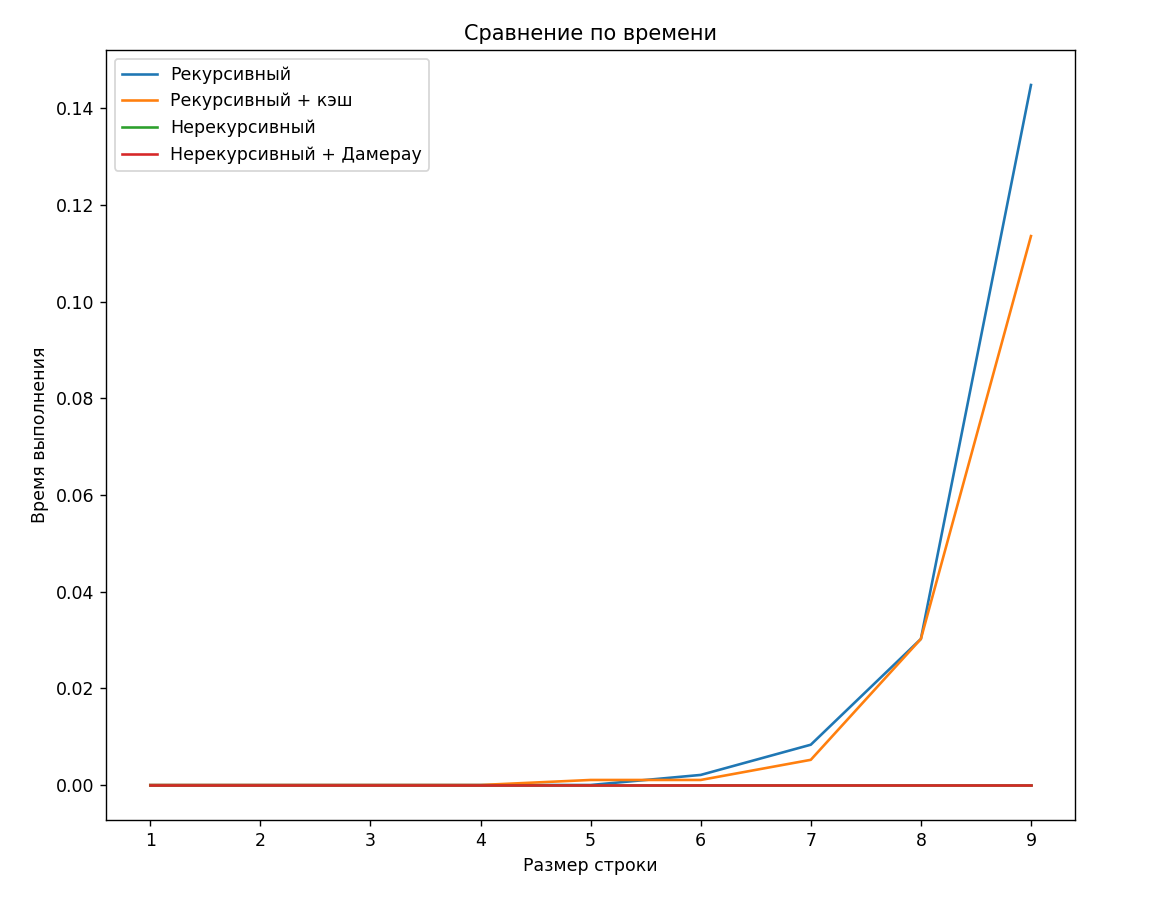
\includegraphics[scale=0.7]{tools/Screenshot_1.png}
	\caption{Сравнение алгоритмов по времени выполнения}
\end{figure}

\begin{table}[h]
	\begin{center}
	\caption{\label{tbl:time_cmp} Сравнение нерекурсивных алгоритмов по времени выполнения}
	\begin{tabular}{|c|c|c|}
		\hline
		Размер строк & Левенштейн & Дамерау-Левенштейн
		\\ \hline
		50 & 0 & 0
		\\ \hline
		100 & 0.001 & 0.001
		\\ \hline
		150 & 0.002 & 0.001
		\\ \hline
		200 & 0.002 & 0.003
		\\ \hline
		250 & 0.005 & 0.007
		\\ \hline
		300 & 0.008 & 0.009
		\\ \hline
		350 & 0.015 & 0.016
		\\ \hline
		400 & 0.016 & 0.022
		\\ \hline
	\end{tabular}
	\end{center}
\end{table}

\clearpage\begin{figure}[h]
	\centering
	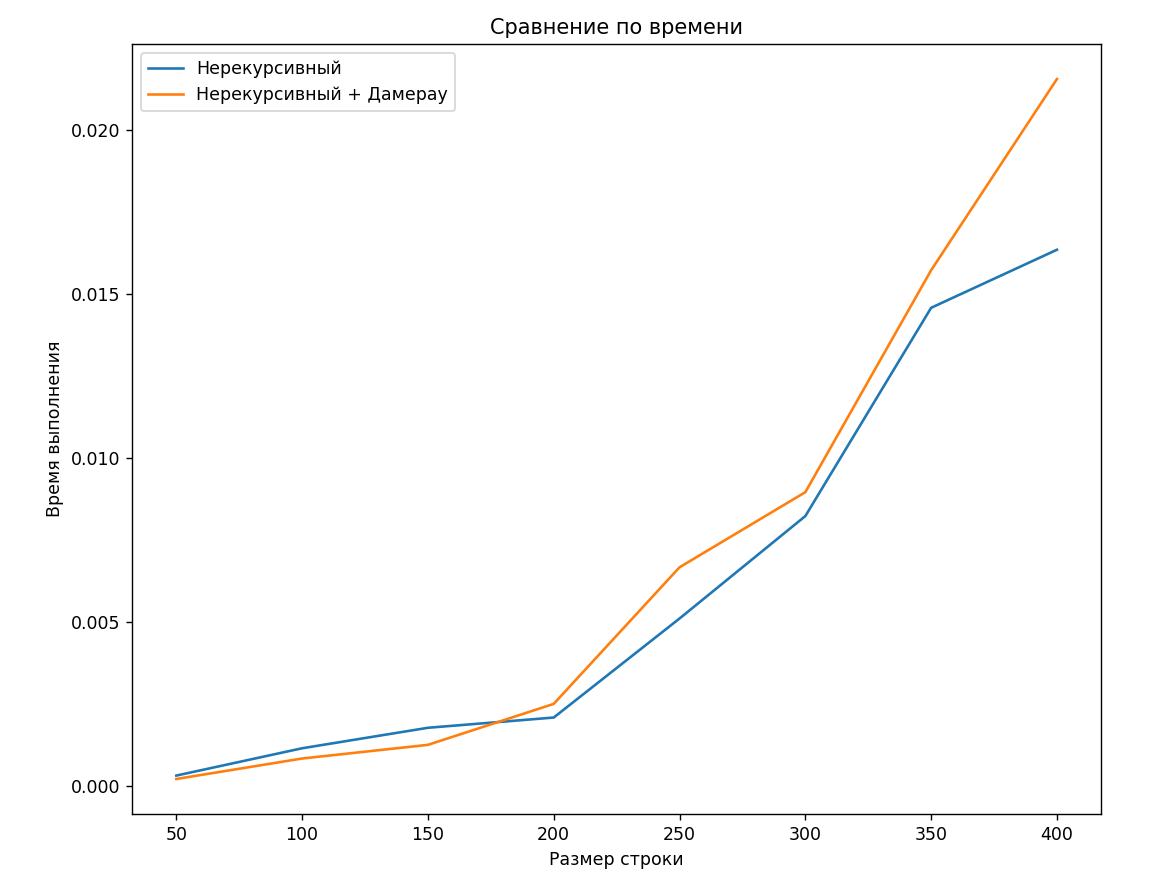
\includegraphics[scale=0.7]{tools/Screenshot_2.png}
	\caption{Сравнение нерекурсивных алгоритмов по времени выполнения}
\end{figure}

\subsection{Сравнение по памяти}
В таблице \ref{tbl:mem_comp} приведено сравнение различных реализаций по памяти. Нерекурсивные алгоритмы
Левенштейна и Дамерау-Левенштейна эквивалентны по расходу памяти.
\clearpage\begin{table}[h]
	\begin{center}
	\caption{\label{tbl:mem_comp} Сравнение по памяти двух строк длины N и M соответственно}
	\begin{tabular}{|c|c|c|c|c|}
		\hline
		N & M & Рекурсивно, байт &  Рекурсивно + кэш, байт & Нерекурсивно, байт
		\\ \hline
		10 & 10 & 20 & 141 & 141
		\\ \hline
		100 & 100 & 200 & 10401 & 10401
		\\ \hline
		200 & 200 & 400 & 40801 & 40801
		\\ \hline
		500 & 500 & 1000 & 252001 & 252001
		\\ \hline
		1000 & 1000 & 2000 & 1004001 & 1004001
		\\ \hline
		n & m & n + m & n * m + n + m & n * m + n + m
		\\ \hline
	\end{tabular}
	\end{center}
\end{table}

\subsection{Вывод}
Рекурсивные алгоритмы работают намного дольше, чем нерекурсивные  алгоритмы, в силу большей сложности.
Алгоритм с кэшем дает небольшое преимущество перед простым рекурсивным алгоритмом, так как выполняет
меньше рекурсивных вызовов. Простой рекурсивный алгоритм расходует меньше  памяти, чем все остальные,
потому что не хранит дополнительную матрицу. Нерекурсивный алгоритм Дамерау-Левенштейна медленнее, чем 
нерекурсивный алгоритм Левенштейна, в силу появления дополнительного сравнения на возможность обмена
двух символов строки.


\clearpage\section*{Заключение}
\addcontentsline{toc}{section}{ЗАКЛЮЧЕНИЕ}
В ходе выполнения лабораторной работы поставленная цель была достигнута, а также были решены следующие задачи:
\begin{itemize}
	\item изучены алгоритмы Левенштейна и Дамерау-Левенштейна
	\item реализованы алгоритмы на языке $Python$ 
	\item проведено сравнение алгоритмов по времени и памяти
	\item описаны и обоснованы полученные результаты
\end{itemize} 

\renewcommand{\bibname}{Список использованной литературы}
\clearpage\begin{thebibliography}{4}
	\bibitem{bib1}
	process\_time --  https://docs.python.org/3/library/time.html\#functions
	\bibitem{bib2}
	Welcome to Python -- https://www.python.org
	\bibitem{bib3}
	Библиотека time -- https://docs.python.org/3/library/time.html
	\bibitem{bib4}
	Левенштейн В. И. Двоичные коды с исправлением выпадений, вставок и замещений символов. – М.: Доклады АН 
	СССР, 1965. Т. 163. С. 845– 848.
\end{thebibliography}
\addcontentsline{toc}{section}{СПИСОК ИСПОЛЬЗОВАННОЙ ЛИТЕРАТУРЫ}

\end{document}